% Chapter 4
\chapter{SYSTEM DESIGN} % All Chapter headings in ALL CAPS


\section{Components in the project}
\subsection{Hardware Components}
\begin{verbatim}
1. Raspberry Pi 2 microcomputer
2. 9DOF IMU Sensor
3. 4 BLDC Motors
4. Raspberry Pi Camera Module
5. 4 Carbon Fibre Propellers
6. Battery
7. Quadcopter Frame
8. ESC
9. Male-Female Connecting Wires
10.4 Propeller Guards
11.Breadboard
12.Resistors
13.Portable Charger
\end{verbatim}
\subsection{Software Components}
\begin{verbatim}
1. Raspbian OS – Jessie
2. OpenCV 3.1.0
3. Python 2.7.6
4. Android Studio IDE
\end{verbatim}
\subsection{Programs}
\begin{verbatim}
a) Python programs to control the quadcopter:
1. PID Controller
2. Kalman Filter
3. Quadcopter Control
4. Python Server
b) Python programs for Panorama Stitching:
1. Camera Calibration
2. Panorama Stitching
c) Python Programs for 3D Reconstruction:
1. Extract Metadata
2. Detect Features
3. Match Features
4. Create Tracks
5. Reconstruct
6. Mesh
d) HTML Code for Visualizing Sparse Reconstruction
e) Android App providing virtual joystick interface
\end{verbatim}

\section{Technology used}
\subsection{Raspberry Pi 2 Microcomputer}
The quadcopter is controlled using the Raspberry Pi 2. Raspberry pi (RPI) is a credit card sized microcomputer that runs on a Linux based operating system loaded on its SD card . It includes a 900MHz quad-core ARM Cortex-A7 CPU and 1GB RAM.
It can connect to a network by using an external user-supplied USB Ethernet or WiFi adapter. Furthermore, the RPi has four USB ports, a full HDMI port, 40 GPIO pins and an Ethernet port. Apart from this, the Raspberry Pi has a camera interface which allows a native Pi Camera to be configured and used. It also has a Micro SD Card slot. The advantage of using a RPi over traditional Arduino boards is that the Pi has much greater computational power and thus, more complicated and better stabilization algorithms can be run on it. 

\begin{figure}[H]
  \centering
  \includegraphics[width = 15cm, height = 12cm]{rpi2.jpg}
  \caption{Raspberry Pi}
  \label{RPi}	
\end{figure}

\begin{figure}[H]
  \centering
  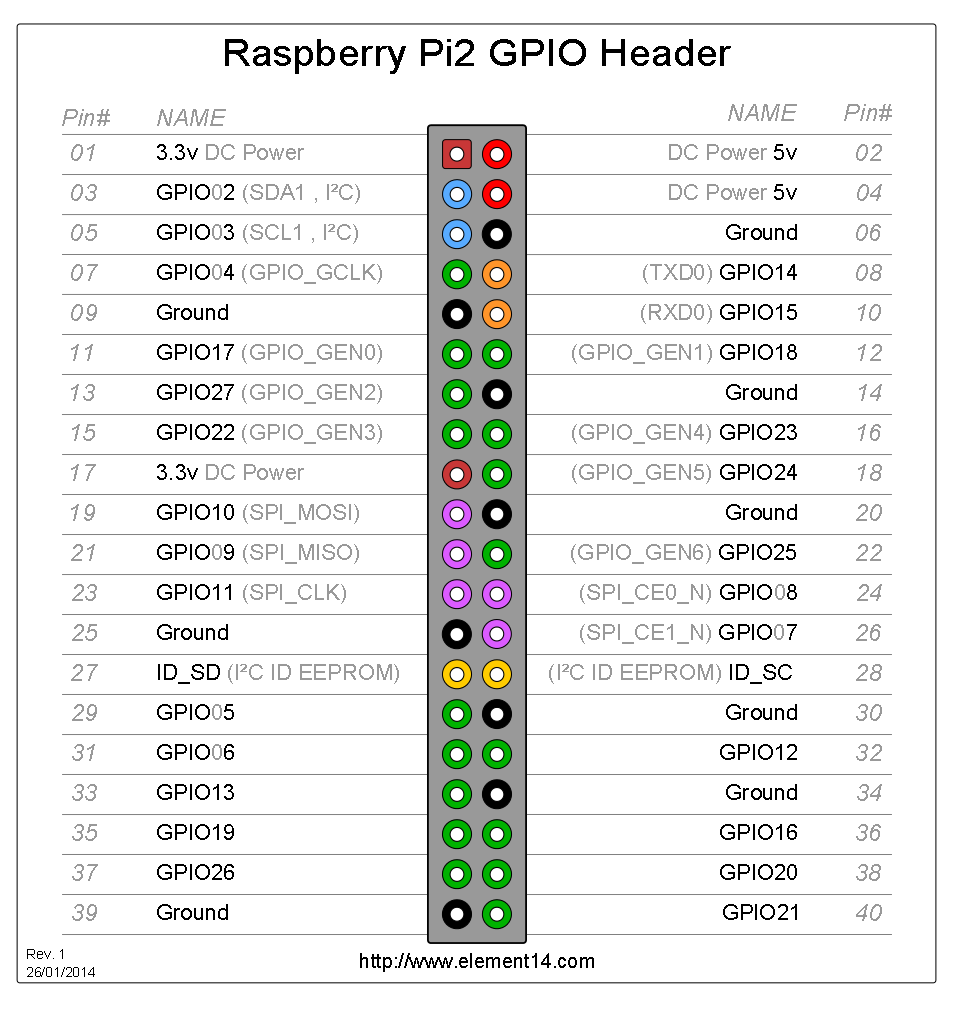
\includegraphics[width = 15cm, height = 12cm]{gpio_header.png}
  \caption{Raspberry Pi 2 GPIO Header}
  \label{RPi Pins} 
\end{figure}


\subsection{Electronic Speed Controller (ESC)}
The Electronic Speed Controller is a circuit which varies the motor's speed, direction and acts like a dynamic brake. ESCs are most often used with BLDC motors necessary for translating digital signals to electric current. ESCs are an essential component of modern multirotor crafts that offer high power, high frequency, high resolution 3-phase AC power to the motors in an extremely compact miniature package. These crafts depend entirely on the variable speed of the motors driving the propellers. The large variation and fine RPM control in motor/propeller speed gives all of the control necessary for a quadcopter (and all multirotors) to fly. On a quadcopter, each motor gets its own ESC, each of which connects to the controller. After computing the inputs(the amount of current and direction to be given to each motor), the controller directs each ESC to adjust its speed according to the PWM signal provided.
This quadcopter uses a 40A, 3s ESC.
\begin{figure}[H]
  \centering
  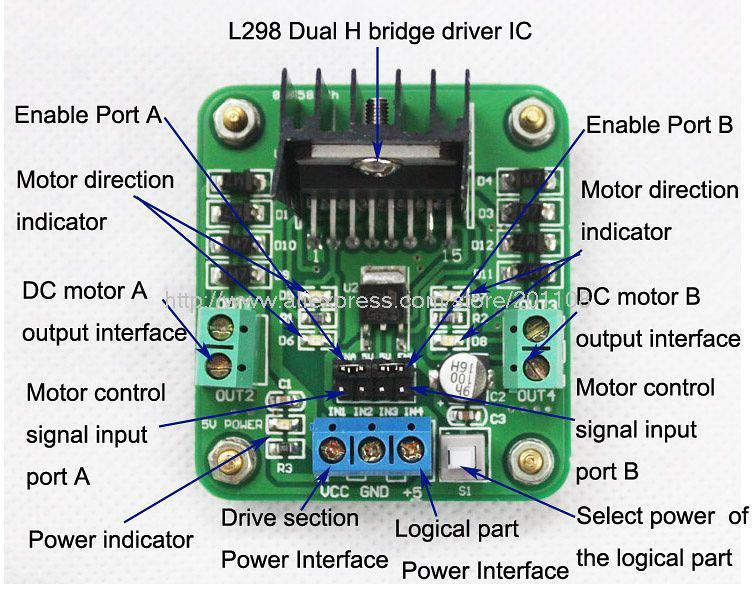
\includegraphics[width = 15cm, height = 12cm]{motor.jpg}
  \caption{40A 3s ESC}
  \label{40A 3s ESC}	
\end{figure}



\subsection{IMU Sensor}
An inertial measurement unit (IMU) is an electronic device that measures and reports a body's specific force, angular rate, and sometimes the magnetic field surrounding the body, using a combination of accelerometers and gyroscopes and magnetometers. IMUs are typically used to maneuver aircraft, including UAVs. This project uses a 9DOF IMU sensor with a 3-axis accelerometer, 3-axis gyroscope and 3-axis magnetometer. The accelerometer measures acceleration and has high accuracy. The gyroscope measures the angular velocity and is used to stabilize flight. It is less accurate than the accelerometer and is prone to drift errors. 
\begin{figure}[H]
  \centering
  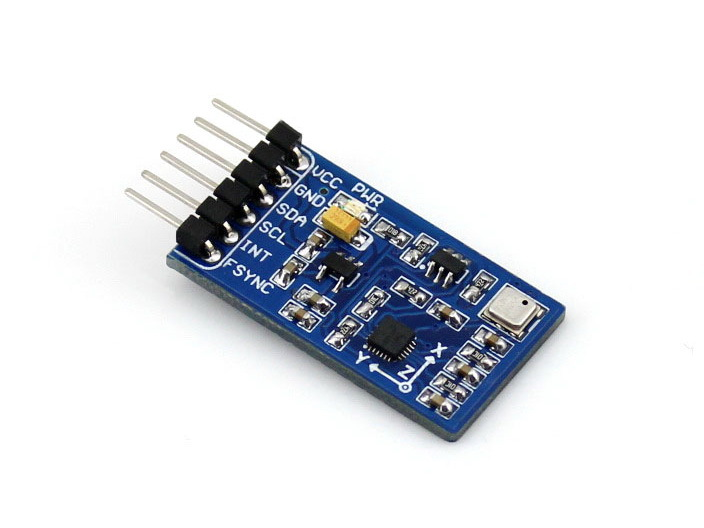
\includegraphics[width = 13cm, height = 7cm]{IMU.jpg}
  \caption{IMU Sensor}
  \label{IMU Sensor}	
\end{figure}

\subsection{Raspberry Pi Camera}
The Raspberry Pi camera module can be used to take high-definition video, as well as photographs. The camera has a five megapixel fixed-focus camera that supports 1080p30, 720p60 and VGA90 video modes, as well as stills capture. It attaches via a 15cm ribbon cable to the CSI port on the Raspberry Pi. It can be configured using the Python Picamera library. The project uses the Pi Camera to capture images for panorama stitching and 3D reconstruction.
\begin{figure}[H]
  \centering
  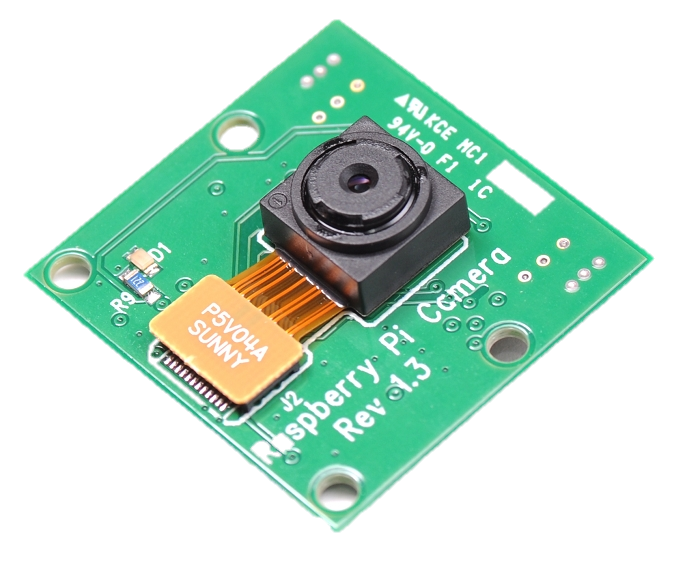
\includegraphics[width = 7cm, height = 6cm]{picam.png}
  \caption{Raspberry Pi camera}
  \label{RPi camera}	
\end{figure}

\section{Block Diagram}

\begin{figure}[H]
  \centering
  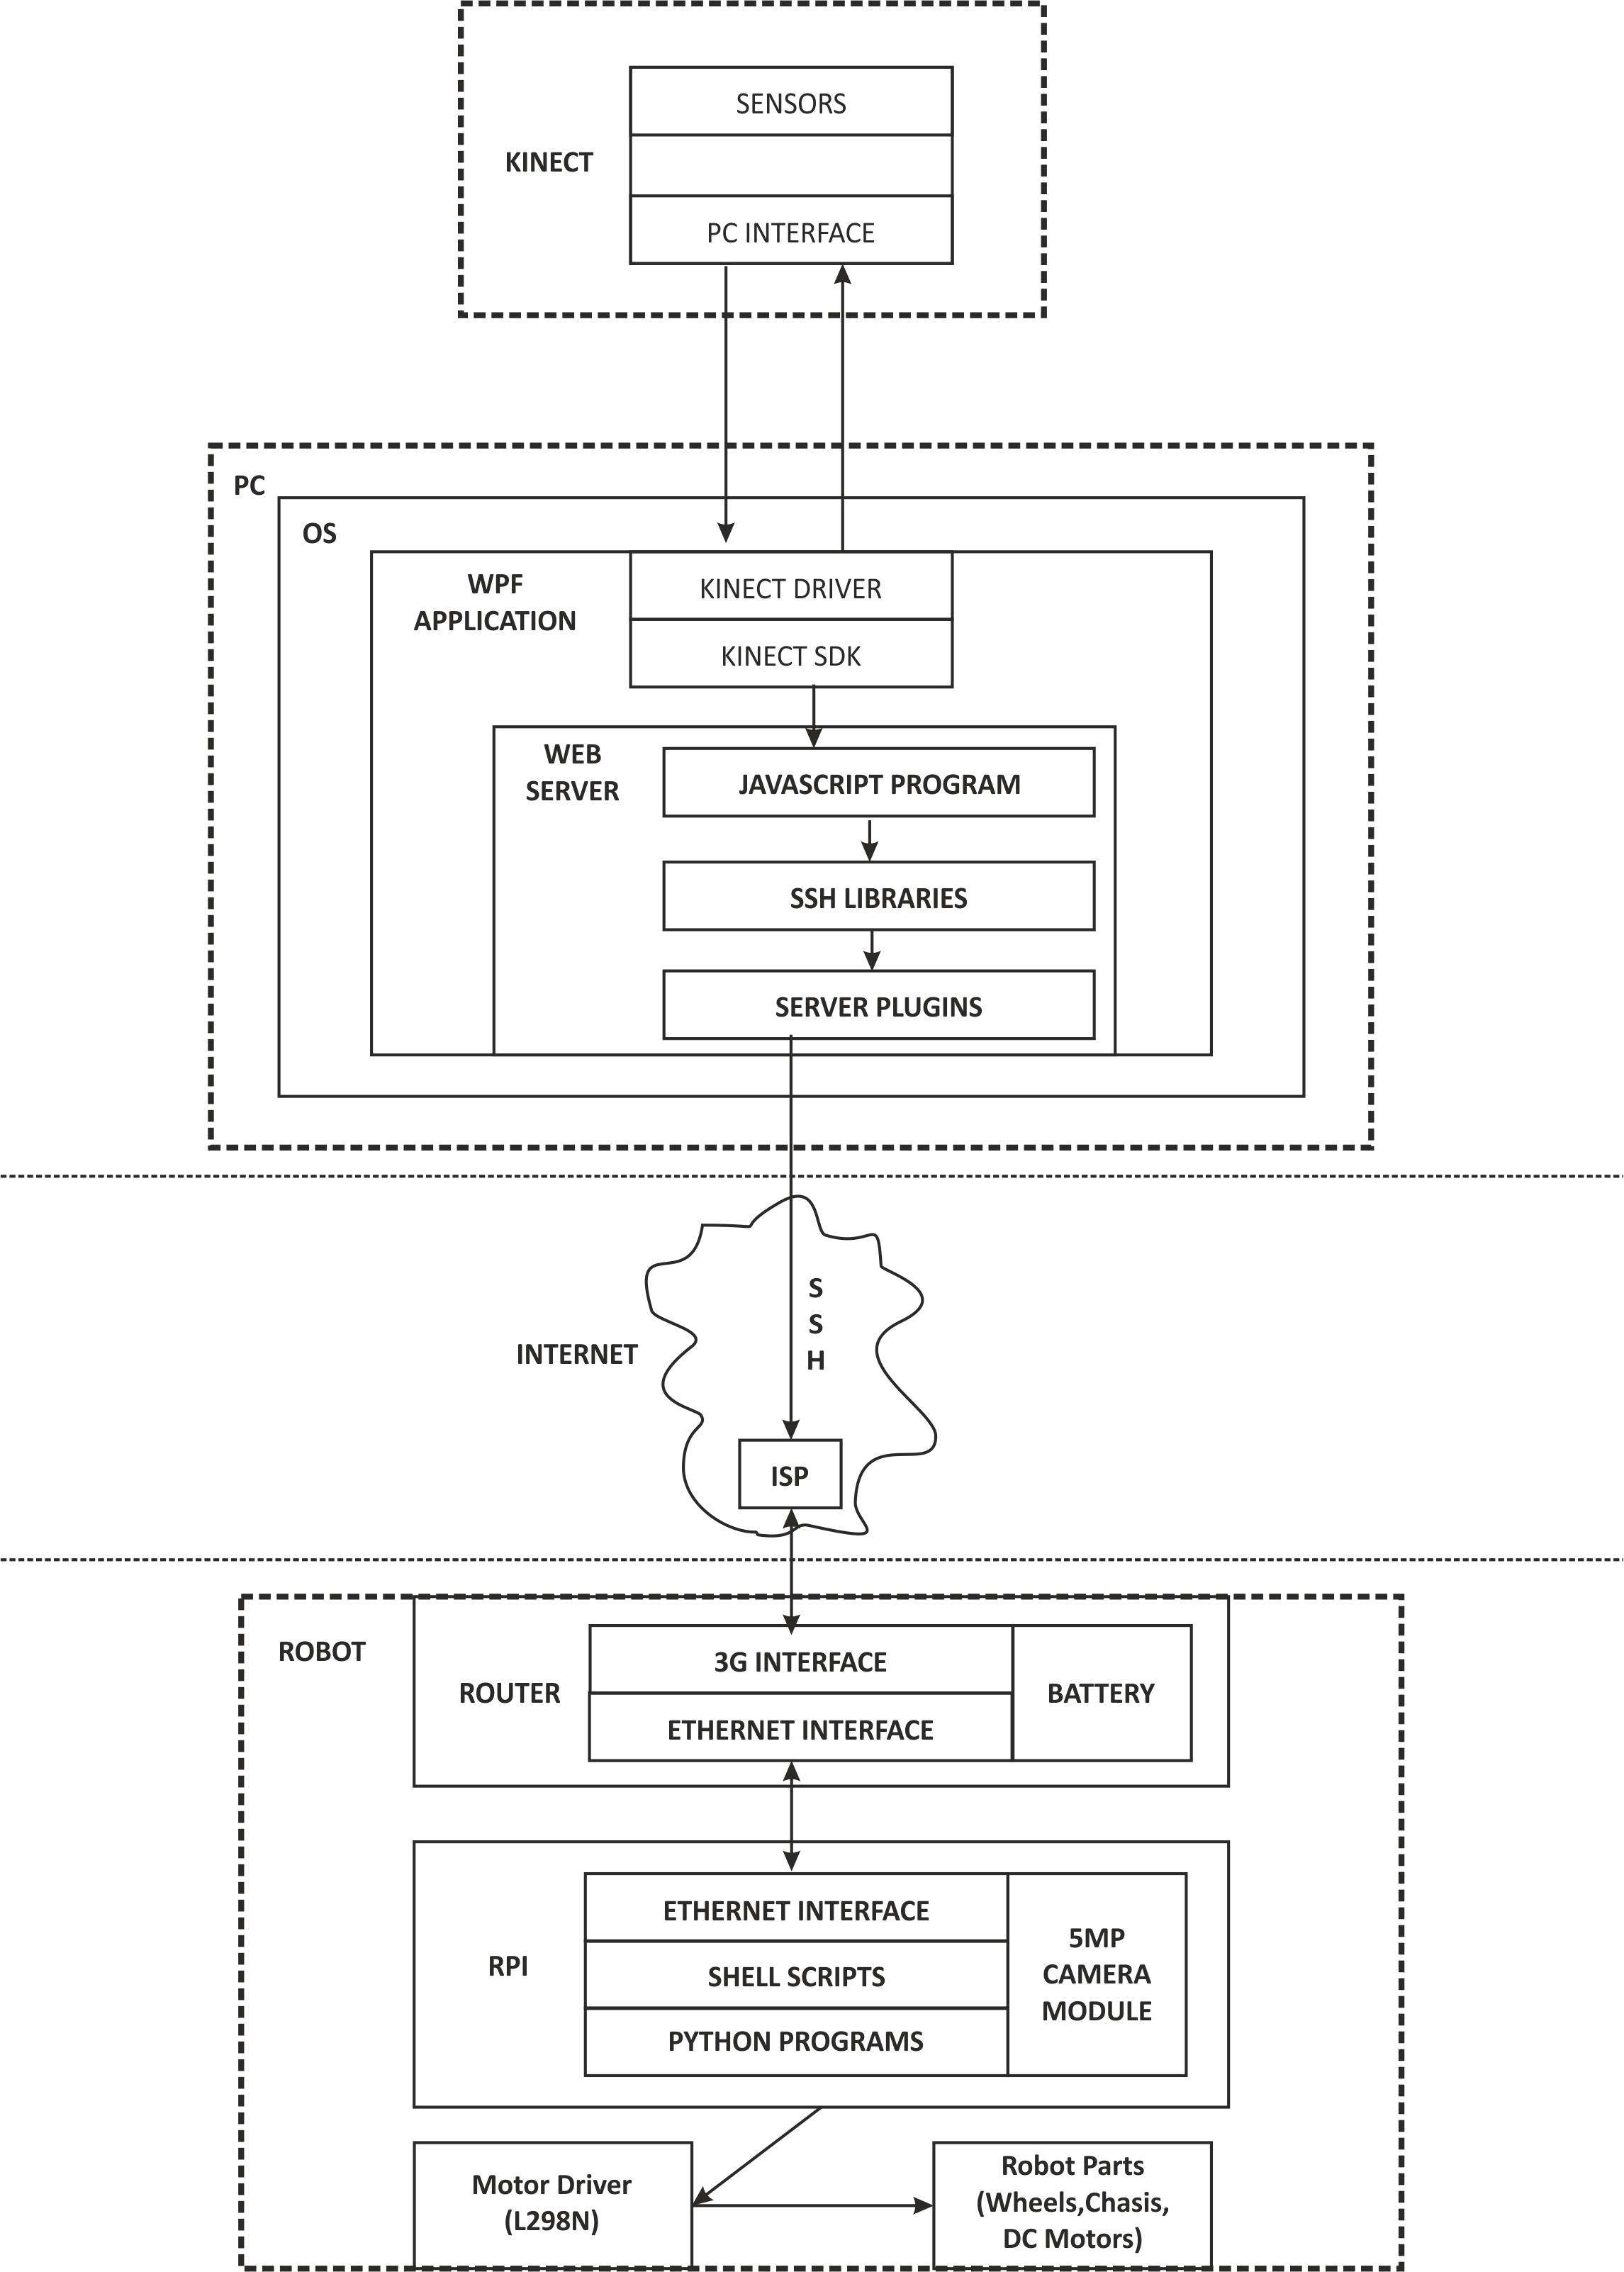
\includegraphics[width = 16cm, height = 16cm]{Blocks.jpg}
  \caption{Block Digram}
  \label{block}	
\end{figure}

\section{Circuit Diagram}

\begin{figure}[H]
  \centering
  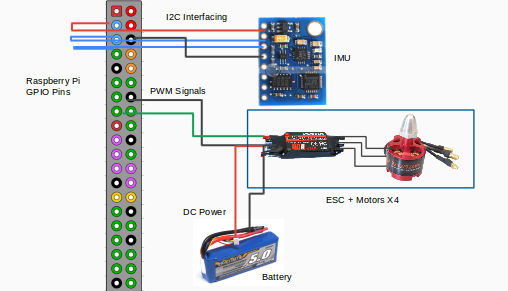
\includegraphics[width = 16cm, height = 16cm]{circuit_dgm.png}
  \caption{Circuit Digram}
  \label{circuit} 
\end{figure}


\section{Flow Diagram}
\begin{figure}[H]
  \centering
  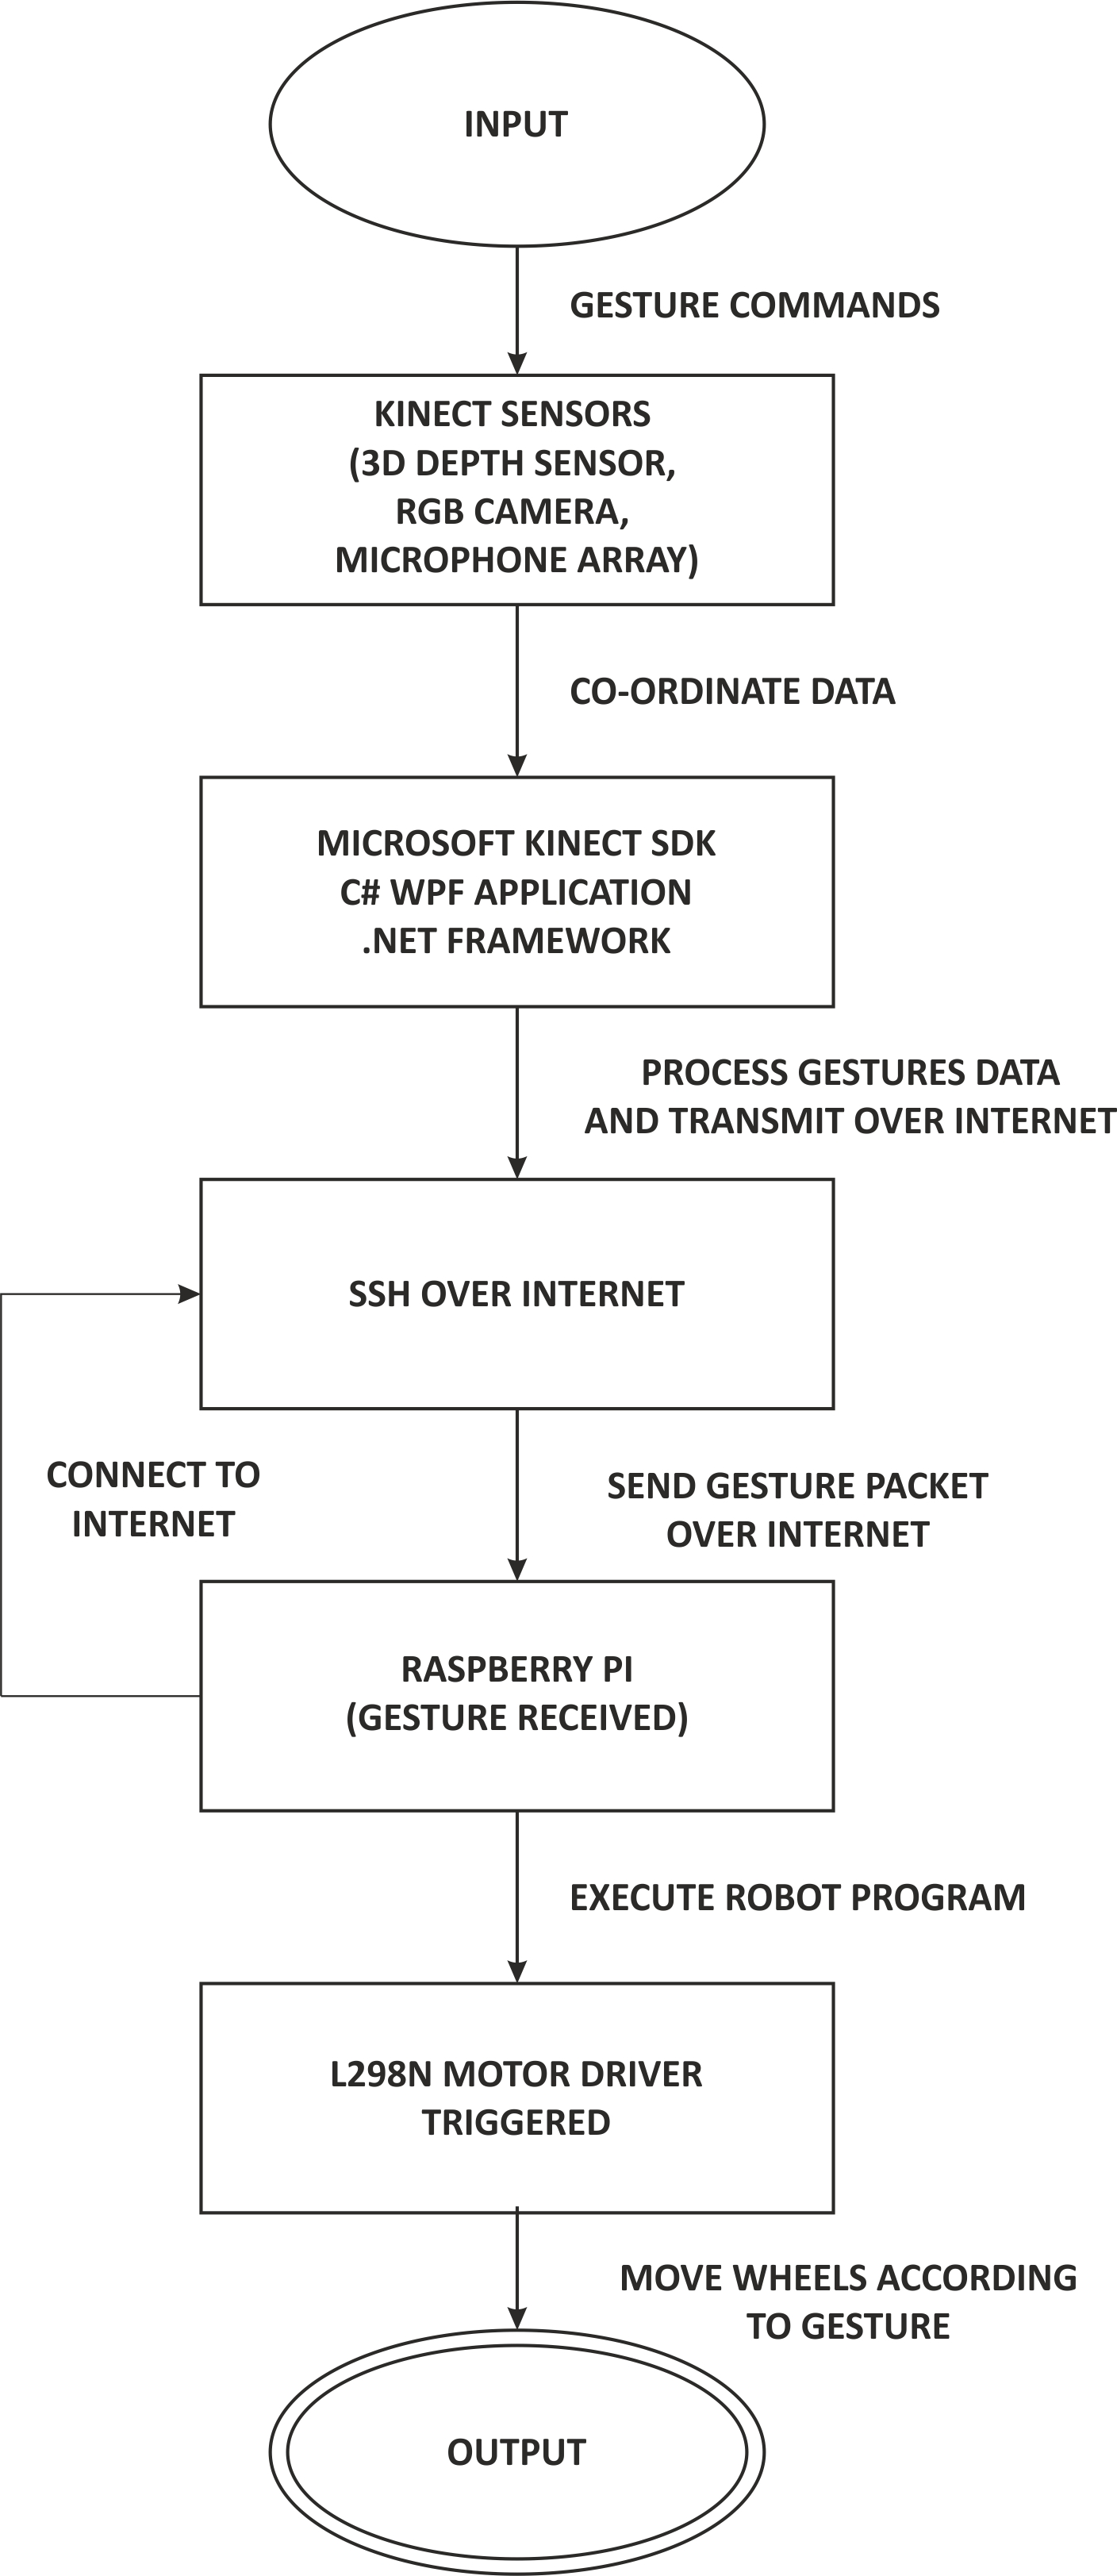
\includegraphics[width = 16cm, height = 19cm]{Flows.jpg}
  \caption{Flow Diagram from Input to Output}
  \label{Flow}	
\end{figure}

\textbf{Description of Flow Diagram}
\newline
The user begins the quadcopter program by clicking a button on the Android App which is sent as input to the Python server on the Raspberry Pi. These signals are sent over a WiFi network using an Android phone as a mobile hotspot. The user can control the altitude of the drone and the individual motors using the virtual Joystick on the app. Signals are sent as JSON-encoded data to the quadcopter. The orientation data i.e. the roll, pitch and yaw values are detected by the IMU sensor on the quadcopter and are fed as input to the balancing algorithm. This data is processed by the python program and the orientation of the quadcopter is automatically corrected using the PID algorithm. When the camera signal is triggered, the Pi Camera begins taking pictures at an interval of 1 second and saves them on the SD Card. Once the camera is disabled, the image-processing program is executed on the captured images. The final results i.e. the Panorama image and the reconstructed 3D Point Cloud are separately rendered on a web browser using a remote laptop on the ground. Thus, the quadcopter is semi-autonomous as its flight is controlled by the user but its stability is automatically corrected. It is remotely controlled using an Android app.



